% Options for packages loaded elsewhere
\PassOptionsToPackage{unicode}{hyperref}
\PassOptionsToPackage{hyphens}{url}
%
\documentclass[
]{article}
\usepackage{lmodern}
\usepackage{amssymb,amsmath}
\usepackage{ifxetex,ifluatex}
\ifnum 0\ifxetex 1\fi\ifluatex 1\fi=0 % if pdftex
  \usepackage[T1]{fontenc}
  \usepackage[utf8]{inputenc}
  \usepackage{textcomp} % provide euro and other symbols
\else % if luatex or xetex
  \usepackage{unicode-math}
  \defaultfontfeatures{Scale=MatchLowercase}
  \defaultfontfeatures[\rmfamily]{Ligatures=TeX,Scale=1}
\fi
% Use upquote if available, for straight quotes in verbatim environments
\IfFileExists{upquote.sty}{\usepackage{upquote}}{}
\IfFileExists{microtype.sty}{% use microtype if available
  \usepackage[]{microtype}
  \UseMicrotypeSet[protrusion]{basicmath} % disable protrusion for tt fonts
}{}
\makeatletter
\@ifundefined{KOMAClassName}{% if non-KOMA class
  \IfFileExists{parskip.sty}{%
    \usepackage{parskip}
  }{% else
    \setlength{\parindent}{0pt}
    \setlength{\parskip}{6pt plus 2pt minus 1pt}}
}{% if KOMA class
  \KOMAoptions{parskip=half}}
\makeatother
\usepackage{xcolor}
\IfFileExists{xurl.sty}{\usepackage{xurl}}{} % add URL line breaks if available
\IfFileExists{bookmark.sty}{\usepackage{bookmark}}{\usepackage{hyperref}}
\hypersetup{
  pdftitle={lab file 7},
  pdfauthor={Jack Wright},
  hidelinks,
  pdfcreator={LaTeX via pandoc}}
\urlstyle{same} % disable monospaced font for URLs
\usepackage[margin=1in]{geometry}
\usepackage{color}
\usepackage{fancyvrb}
\newcommand{\VerbBar}{|}
\newcommand{\VERB}{\Verb[commandchars=\\\{\}]}
\DefineVerbatimEnvironment{Highlighting}{Verbatim}{commandchars=\\\{\}}
% Add ',fontsize=\small' for more characters per line
\usepackage{framed}
\definecolor{shadecolor}{RGB}{248,248,248}
\newenvironment{Shaded}{\begin{snugshade}}{\end{snugshade}}
\newcommand{\AlertTok}[1]{\textcolor[rgb]{0.94,0.16,0.16}{#1}}
\newcommand{\AnnotationTok}[1]{\textcolor[rgb]{0.56,0.35,0.01}{\textbf{\textit{#1}}}}
\newcommand{\AttributeTok}[1]{\textcolor[rgb]{0.77,0.63,0.00}{#1}}
\newcommand{\BaseNTok}[1]{\textcolor[rgb]{0.00,0.00,0.81}{#1}}
\newcommand{\BuiltInTok}[1]{#1}
\newcommand{\CharTok}[1]{\textcolor[rgb]{0.31,0.60,0.02}{#1}}
\newcommand{\CommentTok}[1]{\textcolor[rgb]{0.56,0.35,0.01}{\textit{#1}}}
\newcommand{\CommentVarTok}[1]{\textcolor[rgb]{0.56,0.35,0.01}{\textbf{\textit{#1}}}}
\newcommand{\ConstantTok}[1]{\textcolor[rgb]{0.00,0.00,0.00}{#1}}
\newcommand{\ControlFlowTok}[1]{\textcolor[rgb]{0.13,0.29,0.53}{\textbf{#1}}}
\newcommand{\DataTypeTok}[1]{\textcolor[rgb]{0.13,0.29,0.53}{#1}}
\newcommand{\DecValTok}[1]{\textcolor[rgb]{0.00,0.00,0.81}{#1}}
\newcommand{\DocumentationTok}[1]{\textcolor[rgb]{0.56,0.35,0.01}{\textbf{\textit{#1}}}}
\newcommand{\ErrorTok}[1]{\textcolor[rgb]{0.64,0.00,0.00}{\textbf{#1}}}
\newcommand{\ExtensionTok}[1]{#1}
\newcommand{\FloatTok}[1]{\textcolor[rgb]{0.00,0.00,0.81}{#1}}
\newcommand{\FunctionTok}[1]{\textcolor[rgb]{0.00,0.00,0.00}{#1}}
\newcommand{\ImportTok}[1]{#1}
\newcommand{\InformationTok}[1]{\textcolor[rgb]{0.56,0.35,0.01}{\textbf{\textit{#1}}}}
\newcommand{\KeywordTok}[1]{\textcolor[rgb]{0.13,0.29,0.53}{\textbf{#1}}}
\newcommand{\NormalTok}[1]{#1}
\newcommand{\OperatorTok}[1]{\textcolor[rgb]{0.81,0.36,0.00}{\textbf{#1}}}
\newcommand{\OtherTok}[1]{\textcolor[rgb]{0.56,0.35,0.01}{#1}}
\newcommand{\PreprocessorTok}[1]{\textcolor[rgb]{0.56,0.35,0.01}{\textit{#1}}}
\newcommand{\RegionMarkerTok}[1]{#1}
\newcommand{\SpecialCharTok}[1]{\textcolor[rgb]{0.00,0.00,0.00}{#1}}
\newcommand{\SpecialStringTok}[1]{\textcolor[rgb]{0.31,0.60,0.02}{#1}}
\newcommand{\StringTok}[1]{\textcolor[rgb]{0.31,0.60,0.02}{#1}}
\newcommand{\VariableTok}[1]{\textcolor[rgb]{0.00,0.00,0.00}{#1}}
\newcommand{\VerbatimStringTok}[1]{\textcolor[rgb]{0.31,0.60,0.02}{#1}}
\newcommand{\WarningTok}[1]{\textcolor[rgb]{0.56,0.35,0.01}{\textbf{\textit{#1}}}}
\usepackage{graphicx,grffile}
\makeatletter
\def\maxwidth{\ifdim\Gin@nat@width>\linewidth\linewidth\else\Gin@nat@width\fi}
\def\maxheight{\ifdim\Gin@nat@height>\textheight\textheight\else\Gin@nat@height\fi}
\makeatother
% Scale images if necessary, so that they will not overflow the page
% margins by default, and it is still possible to overwrite the defaults
% using explicit options in \includegraphics[width, height, ...]{}
\setkeys{Gin}{width=\maxwidth,height=\maxheight,keepaspectratio}
% Set default figure placement to htbp
\makeatletter
\def\fps@figure{htbp}
\makeatother
\setlength{\emergencystretch}{3em} % prevent overfull lines
\providecommand{\tightlist}{%
  \setlength{\itemsep}{0pt}\setlength{\parskip}{0pt}}
\setcounter{secnumdepth}{-\maxdimen} % remove section numbering

\title{lab file 7}
\author{Jack Wright}
\date{10/18/2020}

\begin{document}
\maketitle

\begin{Shaded}
\begin{Highlighting}[]
\KeywordTok{library}\NormalTok{(tidyverse)}
\KeywordTok{library}\NormalTok{(openintro)}
\KeywordTok{library}\NormalTok{(infer)}
\end{Highlighting}
\end{Shaded}

\hypertarget{exercise-1}{%
\subsection{Exercise 1}\label{exercise-1}}

The cases are about 13583 school aged children. Remember that you can
answer this question by viewing the data in the data viewer or by using
the following command:

\begin{Shaded}
\begin{Highlighting}[]
\KeywordTok{data}\NormalTok{(yrbss)}
\end{Highlighting}
\end{Shaded}

\hypertarget{exercise-2}{%
\subsection{Exercise 2}\label{exercise-2}}

\begin{enumerate}
\def\labelenumi{\arabic{enumi}.}
\tightlist
\item
  How many observations are we missing weights from?
\end{enumerate}

\begin{Shaded}
\begin{Highlighting}[]
\KeywordTok{summary}\NormalTok{(yrbss}\OperatorTok{$}\NormalTok{weight)}
\end{Highlighting}
\end{Shaded}

\begin{verbatim}
##    Min. 1st Qu.  Median    Mean 3rd Qu.    Max.    NA's 
##   29.94   56.25   64.41   67.91   76.20  180.99    1004
\end{verbatim}

\begin{Shaded}
\begin{Highlighting}[]
\NormalTok{yrbss}\OperatorTok
\StringTok{  }\KeywordTok{filter}\NormalTok{(}\KeywordTok{is.na}\NormalTok{(weight))}\OperatorTok
\StringTok{  }\KeywordTok{nrow}\NormalTok{()}
\end{Highlighting}
\end{Shaded}

\begin{verbatim}
## [1] 1004
\end{verbatim}

1004 cases are missing weights.

\begin{Shaded}
\begin{Highlighting}[]
\NormalTok{yrbss <-}\StringTok{ }\NormalTok{yrbss }\OperatorTok\StringTok{ }
\StringTok{  }\KeywordTok{mutate}\NormalTok{(}\DataTypeTok{physical_3plus =} \KeywordTok{ifelse}\NormalTok{(yrbss}\OperatorTok{$}\NormalTok{physically_active_7d }\OperatorTok{>}\StringTok{ }\DecValTok{2}\NormalTok{, }\StringTok{"yes"}\NormalTok{, }\StringTok{"no"}\NormalTok{))}
\end{Highlighting}
\end{Shaded}

\hypertarget{exercise-3}{%
\subsection{Exercise 3}\label{exercise-3}}

\begin{enumerate}
\def\labelenumi{\arabic{enumi}.}
\tightlist
\item
  Make a side-by-side boxplot of \texttt{physical\_3plus} and
  \texttt{weight}. Is there a relationship between these two variables?
  What did you expect and why?
\end{enumerate}

They look very similar. I was expecting people who were physical 3 times
a week to weigh less on average but the medians look similar as well as
the IQR.

\begin{Shaded}
\begin{Highlighting}[]
\NormalTok{yrbss}\OperatorTok{$}\NormalTok{physical_3plus<-}\KeywordTok{as.factor}\NormalTok{(yrbss}\OperatorTok{$}\NormalTok{physical_3plus)}
\NormalTok{yrb_plot<-yrbss}\OperatorTok
\StringTok{  }\KeywordTok{filter}\NormalTok{(}\OperatorTok{!}\KeywordTok{is.na}\NormalTok{(weight),}\OperatorTok{!}\KeywordTok{is.na}\NormalTok{(physical_3plus))}
\NormalTok{p<-}\KeywordTok{ggplot}\NormalTok{(yrb_plot, }\KeywordTok{aes}\NormalTok{(}\DataTypeTok{x=}\NormalTok{physical_3plus,}\DataTypeTok{y=}\NormalTok{weight))}\OperatorTok{+}
\StringTok{  }\KeywordTok{geom_boxplot}\NormalTok{()}
\NormalTok{p}
\end{Highlighting}
\end{Shaded}

\includegraphics{lab-7-try-3_files/figure-latex/unnamed-chunk-4-1.pdf}

\begin{Shaded}
\begin{Highlighting}[]
\NormalTok{yrbss }\OperatorTok
\StringTok{  }\KeywordTok{group_by}\NormalTok{(physical_3plus) }\OperatorTok
\StringTok{  }\KeywordTok{summarise}\NormalTok{(}\DataTypeTok{mean_weight =} \KeywordTok{mean}\NormalTok{(weight, }\DataTypeTok{na.rm =} \OtherTok{TRUE}\NormalTok{))}
\end{Highlighting}
\end{Shaded}

\begin{verbatim}
## `summarise()` ungrouping output (override with `.groups` argument)
\end{verbatim}

\begin{verbatim}
## # A tibble: 3 x 2
##   physical_3plus mean_weight
##   <fct>                <dbl>
## 1 no                    66.7
## 2 yes                   68.4
## 3 <NA>                  69.9
\end{verbatim}

\hypertarget{exercise-4}{%
\subsection{Exercise 4}\label{exercise-4}}

\begin{enumerate}
\def\labelenumi{\arabic{enumi}.}
\tightlist
\item
  Are all conditions necessary for inference satisfied? Comment on each.
  You can compute the group sizes with the \texttt{summarize} command
  above by defining a new variable with the definition \texttt{n()}
\end{enumerate}

CONDITIONS FOR INFERENCE:

Independence:

it was a SRS and the two groups are not linked, necessarily one who
excersizes 3 times a week plus cannot be in the group that doesn't.

Size:

the groups are less than 10\% of the total population of kids who
excersize and those who don't

in the study\ldots{}

\begin{Shaded}
\begin{Highlighting}[]
\CommentTok{#create new variable n}

\NormalTok{yrbss<-}\StringTok{ }\NormalTok{yrbss }\OperatorTok\StringTok{ }
\StringTok{  }\KeywordTok{mutate}\NormalTok{(}\DataTypeTok{n =} \KeywordTok{ifelse}\NormalTok{(yrbss}\OperatorTok{$}\NormalTok{physically_active_7d }\OperatorTok{>}\StringTok{ }\DecValTok{2}\NormalTok{, }\StringTok{"yes"}\NormalTok{, }\StringTok{"no"}\NormalTok{))}

\NormalTok{yrbss}\OperatorTok{$}\NormalTok{n<-}\KeywordTok{as.factor}\NormalTok{(yrbss}\OperatorTok{$}\NormalTok{n)}

\KeywordTok{view}\NormalTok{(yrbss)}
\NormalTok{yrbss}\OperatorTok
\StringTok{ }\KeywordTok{count}\NormalTok{(n)}
\end{Highlighting}
\end{Shaded}

\begin{verbatim}
## Storing counts in `nn`, as `n` already present in input
## i Use `name = "new_name"` to pick a new name.
\end{verbatim}

\begin{verbatim}
## # A tibble: 3 x 2
##   n        nn
##   <fct> <int>
## 1 no     4404
## 2 yes    8906
## 3 <NA>    273
\end{verbatim}

\hypertarget{exercise-5}{%
\subsection{Exercise 5}\label{exercise-5}}

Hypothesis test:

H\_0: the difference in the means between physical 3 plus and less than
3 are equal (mean1-mean2)=0 H\_A: the weights are diffferent !=0

\begin{Shaded}
\begin{Highlighting}[]
\NormalTok{obs_diff <-}\StringTok{ }\NormalTok{yrbss }\OperatorTok
\StringTok{  }\KeywordTok{specify}\NormalTok{(weight }\OperatorTok{~}\StringTok{ }\NormalTok{physical_3plus) }\OperatorTok
\StringTok{  }\KeywordTok{calculate}\NormalTok{(}\DataTypeTok{stat =} \StringTok{"diff in means"}\NormalTok{, }\DataTypeTok{order =} \KeywordTok{c}\NormalTok{(}\StringTok{"yes"}\NormalTok{, }\StringTok{"no"}\NormalTok{))}
\end{Highlighting}
\end{Shaded}

\begin{verbatim}
## Warning: Removed 1219 rows containing missing values.
\end{verbatim}

\begin{Shaded}
\begin{Highlighting}[]
\NormalTok{null_dist <-}\StringTok{ }\NormalTok{yrbss }\OperatorTok
\StringTok{  }\KeywordTok{specify}\NormalTok{(weight }\OperatorTok{~}\StringTok{ }\NormalTok{physical_3plus) }\OperatorTok
\StringTok{  }\KeywordTok{hypothesize}\NormalTok{(}\DataTypeTok{null =} \StringTok{"independence"}\NormalTok{) }\OperatorTok
\StringTok{  }\KeywordTok{generate}\NormalTok{(}\DataTypeTok{reps =} \DecValTok{1000}\NormalTok{, }\DataTypeTok{type =} \StringTok{"permute"}\NormalTok{) }\OperatorTok
\StringTok{  }\KeywordTok{calculate}\NormalTok{(}\DataTypeTok{stat =} \StringTok{"diff in means"}\NormalTok{, }\DataTypeTok{order =} \KeywordTok{c}\NormalTok{(}\StringTok{"yes"}\NormalTok{, }\StringTok{"no"}\NormalTok{))}
\end{Highlighting}
\end{Shaded}

\begin{verbatim}
## Warning: Removed 1219 rows containing missing values.
\end{verbatim}

\begin{Shaded}
\begin{Highlighting}[]
\KeywordTok{ggplot}\NormalTok{(}\DataTypeTok{data =}\NormalTok{ null_dist, }\KeywordTok{aes}\NormalTok{(}\DataTypeTok{x =}\NormalTok{ stat)) }\OperatorTok{+}
\StringTok{  }\KeywordTok{geom_histogram}\NormalTok{()}
\end{Highlighting}
\end{Shaded}

\begin{verbatim}
## `stat_bin()` using `bins = 30`. Pick better value with `binwidth`.
\end{verbatim}

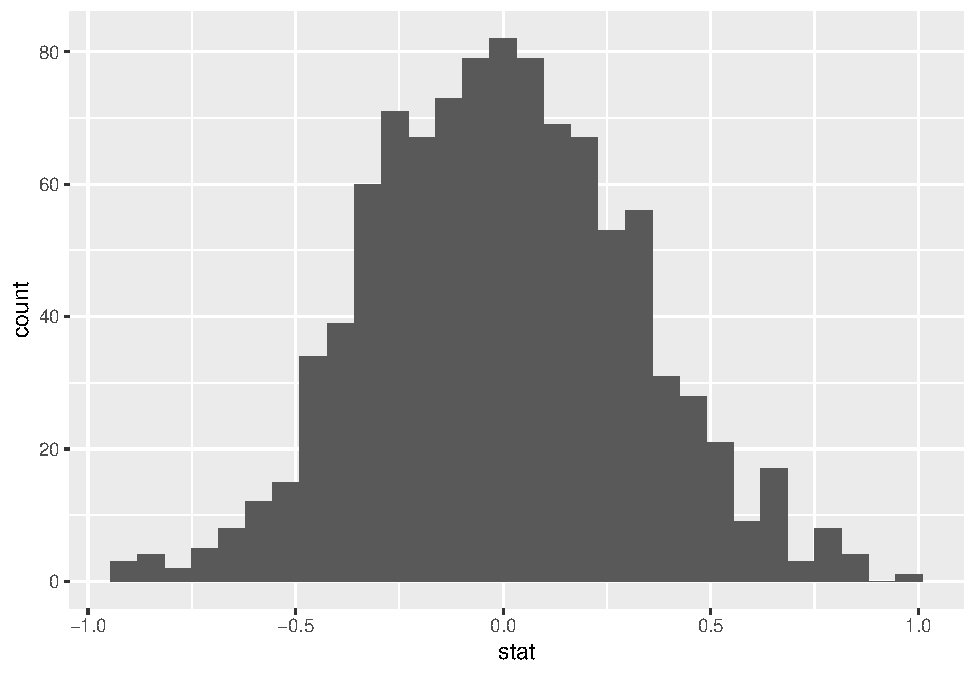
\includegraphics{lab-7-try-3_files/figure-latex/unnamed-chunk-9-1.pdf}

\begin{Shaded}
\begin{Highlighting}[]
\KeywordTok{ggplot}\NormalTok{(}\DataTypeTok{data =}\NormalTok{ null_dist, }\KeywordTok{aes}\NormalTok{(}\DataTypeTok{x =}\NormalTok{ stat)) }\OperatorTok{+}
\StringTok{  }\KeywordTok{geom_histogram}\NormalTok{()}
\end{Highlighting}
\end{Shaded}

\begin{verbatim}
## `stat_bin()` using `bins = 30`. Pick better value with `binwidth`.
\end{verbatim}

\includegraphics{lab-7-try-3_files/figure-latex/unnamed-chunk-10-1.pdf}

\hypertarget{exercise-6}{%
\subsection{Exercise 6}\label{exercise-6}}

\begin{enumerate}
\def\labelenumi{\arabic{enumi}.}
\item
\end{enumerate}

How many of these null permutations have a difference of at least
obs\_stat?

\begin{Shaded}
\begin{Highlighting}[]
\NormalTok{obs_diff_val<-obs_diff}\OperatorTok{$}\NormalTok{stat[}\DecValTok{1}\NormalTok{]}

\NormalTok{null_list<-}\KeywordTok{as.list}\NormalTok{(null_dist}\OperatorTok{$}\NormalTok{stat)}
\NormalTok{null_abs<-}\KeywordTok{lapply}\NormalTok{(null_list, }\DataTypeTok{FUN=}\ControlFlowTok{function}\NormalTok{(x)\{}\KeywordTok{abs}\NormalTok{(x)\})}

\NormalTok{null_dist}\OperatorTok
\StringTok{  }\KeywordTok{summarise}\NormalTok{(}\DataTypeTok{mean=} \KeywordTok{mean}\NormalTok{(stat, }\DataTypeTok{na.rm=}\OtherTok{TRUE}\NormalTok{))}
\end{Highlighting}
\end{Shaded}

\begin{verbatim}
## # A tibble: 1 x 1
##      mean
##     <dbl>
## 1 0.00388
\end{verbatim}

\begin{Shaded}
\begin{Highlighting}[]
\NormalTok{null_dist}\OperatorTok
\StringTok{  }\KeywordTok{filter}\NormalTok{(stat}\OperatorTok{>}\NormalTok{obs_diff_val)}
\end{Highlighting}
\end{Shaded}

\begin{verbatim}
## # A tibble: 0 x 2
## # ... with 2 variables: replicate <int>, stat <dbl>
\end{verbatim}

none of the values are greater than the obs\_diff\_val

\begin{Shaded}
\begin{Highlighting}[]
\NormalTok{null_dist }\OperatorTok
\StringTok{  }\KeywordTok{get_p_value}\NormalTok{(}\DataTypeTok{obs_stat =}\NormalTok{ obs_diff, }\DataTypeTok{direction =} \StringTok{"two_sided"}\NormalTok{)}
\end{Highlighting}
\end{Shaded}

\begin{verbatim}
## Warning: Please be cautious in reporting a p-value of 0. This result is an
## approximation based on the number of `reps` chosen in the `generate()` step. See
## `?get_p_value()` for more information.
\end{verbatim}

\begin{verbatim}
## # A tibble: 1 x 1
##   p_value
##     <dbl>
## 1       0
\end{verbatim}

\hypertarget{exercise-7}{%
\subsection{Exercise 7}\label{exercise-7}}

\begin{enumerate}
\def\labelenumi{\arabic{enumi}.}
\item
\end{enumerate}

Construct and record a confidence interval for the difference between
the weights of those who exercise at least three times a week and those
who don't, and interpret this interval in context of the data.

\begin{Shaded}
\begin{Highlighting}[]
\CommentTok{# number of groups}
\NormalTok{n_}\DecValTok{1}\NormalTok{<-}\DecValTok{8406}
\NormalTok{n_}\DecValTok{2}\NormalTok{<-}\DecValTok{4408}

\NormalTok{x_bar_diff<-}\FloatTok{1.78}
\NormalTok{T_score<-}\KeywordTok{pt}\NormalTok{(.}\DecValTok{025}\NormalTok{,}\DecValTok{4407}\NormalTok{,}\DataTypeTok{lower.tail =} \OtherTok{FALSE}\NormalTok{)}\OperatorTok{*}\DecValTok{2}

\CommentTok{#get sigmas of samples}
\NormalTok{sigma_}\DecValTok{1}\NormalTok{<-yrbss }\OperatorTok
\StringTok{  }\KeywordTok{group_by}\NormalTok{(physical_3plus) }\OperatorTok
\StringTok{  }\KeywordTok{summarise}\NormalTok{(}\DataTypeTok{sd =} \KeywordTok{sd}\NormalTok{(weight, }\DataTypeTok{na.rm =} \OtherTok{TRUE}\NormalTok{))}\OperatorTok
\StringTok{  }\KeywordTok{filter}\NormalTok{(physical_3plus}\OperatorTok{==}\StringTok{"yes"}\NormalTok{)}\OperatorTok
\StringTok{  }\KeywordTok{select}\NormalTok{(sd)}\OperatorTok
\StringTok{  }\KeywordTok{as.double}\NormalTok{()}
\end{Highlighting}
\end{Shaded}

\begin{verbatim}
## `summarise()` ungrouping output (override with `.groups` argument)
\end{verbatim}

\begin{Shaded}
\begin{Highlighting}[]
\NormalTok{sigma_}\DecValTok{2}\NormalTok{<-yrbss }\OperatorTok
\StringTok{  }\KeywordTok{group_by}\NormalTok{(physical_3plus) }\OperatorTok
\StringTok{  }\KeywordTok{summarise}\NormalTok{(}\DataTypeTok{sd =} \KeywordTok{sd}\NormalTok{(weight, }\DataTypeTok{na.rm =} \OtherTok{TRUE}\NormalTok{))}\OperatorTok
\StringTok{  }\KeywordTok{filter}\NormalTok{(physical_3plus}\OperatorTok{==}\StringTok{"no"}\NormalTok{)}\OperatorTok
\StringTok{  }\KeywordTok{select}\NormalTok{(sd)}\OperatorTok
\StringTok{  }\KeywordTok{as.double}\NormalTok{()}
\end{Highlighting}
\end{Shaded}

\begin{verbatim}
## `summarise()` ungrouping output (override with `.groups` argument)
\end{verbatim}

\begin{Shaded}
\begin{Highlighting}[]
\NormalTok{SE<-}\KeywordTok{sqrt}\NormalTok{((sigma_}\DecValTok{1}\OperatorTok{^}\DecValTok{2} \OperatorTok{/}\NormalTok{n_}\DecValTok{1}\NormalTok{)}\OperatorTok{+}\NormalTok{(sigma_}\DecValTok{2}\OperatorTok{^}\DecValTok{2}\OperatorTok{/}\NormalTok{n_}\DecValTok{2}\NormalTok{))}

\NormalTok{bot<-x_bar_diff}\OperatorTok{-}\NormalTok{T_score}\OperatorTok{*}\NormalTok{SE}
\NormalTok{top<-x_bar_diff}\OperatorTok{+}\NormalTok{T_score}\OperatorTok{*}\NormalTok{SE}

\KeywordTok{cat}\NormalTok{(}\StringTok{"the 95% confidence interval for comparing the differnece between the means of these two independent samples is "}\NormalTok{,bot,}\StringTok{"to"}\NormalTok{,top)}
\end{Highlighting}
\end{Shaded}

\begin{verbatim}
## the 95% confidence interval for comparing the differnece between the means of these two independent samples is  1.465649 to 2.094351
\end{verbatim}

I am not sure I fully understand the role of the null distribution that
we calculated. This is a little backwards than I thought it would work
but, maybe we can say, since H\_0: there is NO difference bewteen the
two groups falls OUTSIDE our 95\% confidence interval, we can REJECT the
null hypothesis.

\hypertarget{exercise-8}{%
\subsection{Exercise 8}\label{exercise-8}}

\begin{enumerate}
\def\labelenumi{\arabic{enumi}.}
\item
\end{enumerate}

Calculate a 95\% confidence interval for the average height in meters
(height) and interpret it in context.

Explore height

\begin{Shaded}
\begin{Highlighting}[]
\KeywordTok{summary}\NormalTok{(yrbss}\OperatorTok{$}\NormalTok{height)}
\end{Highlighting}
\end{Shaded}

\begin{verbatim}
##    Min. 1st Qu.  Median    Mean 3rd Qu.    Max.    NA's 
##   1.270   1.600   1.680   1.691   1.780   2.110    1004
\end{verbatim}

\begin{Shaded}
\begin{Highlighting}[]
\NormalTok{height<-yrbss}\OperatorTok
\StringTok{  }\KeywordTok{filter}\NormalTok{(}\OperatorTok{!}\KeywordTok{is.na}\NormalTok{(height))}\OperatorTok
\StringTok{  }\KeywordTok{select}\NormalTok{(height)}

\NormalTok{n<-}\KeywordTok{nrow}\NormalTok{(height)}
\NormalTok{df<-n}\DecValTok{-1}
\NormalTok{height<-height}\OperatorTok{$}\NormalTok{height}


\NormalTok{x_bar<-}\KeywordTok{mean}\NormalTok{(height)}
\NormalTok{sigma<-}\KeywordTok{sd}\NormalTok{(height)}
\NormalTok{SE<-sigma}\OperatorTok{/}\KeywordTok{sqrt}\NormalTok{(n)}
\NormalTok{t_star<-}\KeywordTok{qt}\NormalTok{(.}\DecValTok{025}\NormalTok{,}\DataTypeTok{df=}\NormalTok{df)}

\CommentTok{#confidence interval}

\NormalTok{bot<-x_bar}\OperatorTok{-}\KeywordTok{abs}\NormalTok{(t_star}\OperatorTok{*}\NormalTok{SE)}
\NormalTok{top<-x_bar}\OperatorTok{+}\KeywordTok{abs}\NormalTok{(t_star}\OperatorTok{*}\NormalTok{SE)}

\KeywordTok{cat}\NormalTok{(}\StringTok{"the 95% confidence interval is "}\NormalTok{,bot,}\StringTok{" to "}\NormalTok{,top)}
\end{Highlighting}
\end{Shaded}

\begin{verbatim}
## the 95% confidence interval is  1.689411  to  1.693071
\end{verbatim}

\begin{Shaded}
\begin{Highlighting}[]
\NormalTok{t_star<-}\KeywordTok{abs}\NormalTok{(}\KeywordTok{qt}\NormalTok{(.}\DecValTok{05}\NormalTok{,}\DataTypeTok{df=}\NormalTok{df))}
\CommentTok{# the rest is the same}
\NormalTok{x_bar<-}\KeywordTok{mean}\NormalTok{(height)}
\NormalTok{sigma<-}\KeywordTok{sd}\NormalTok{(height)}
\NormalTok{SE<-sigma}\OperatorTok{/}\KeywordTok{sqrt}\NormalTok{(n)}
\NormalTok{bot_}\DecValTok{1}\NormalTok{<-x_bar}\OperatorTok{-}\KeywordTok{abs}\NormalTok{(t_star}\OperatorTok{*}\NormalTok{SE)}
\NormalTok{top_}\DecValTok{1}\NormalTok{<-x_bar}\OperatorTok{+}\KeywordTok{abs}\NormalTok{(t_star}\OperatorTok{*}\NormalTok{SE)}

\KeywordTok{cat}\NormalTok{(}\StringTok{"the 90% confidence interval is "}\NormalTok{,bot_}\DecValTok{1}\NormalTok{,}\StringTok{" to "}\NormalTok{,top_}\DecValTok{1}\NormalTok{)}
\end{Highlighting}
\end{Shaded}

\begin{verbatim}
## the 90% confidence interval is  1.689705  to  1.692777
\end{verbatim}

The difference is so slight, could this be due to the really tight
standard error due to the sample size?

\begin{Shaded}
\begin{Highlighting}[]
\NormalTok{yrbss<-}\KeywordTok{as.data.frame}\NormalTok{(yrbss)}
\KeywordTok{ggplot}\NormalTok{(yrbss, }\KeywordTok{aes}\NormalTok{(}\DataTypeTok{x=}\NormalTok{height))}\OperatorTok{+}
\StringTok{  }\KeywordTok{geom_histogram}\NormalTok{()}
\end{Highlighting}
\end{Shaded}

\begin{verbatim}
## `stat_bin()` using `bins = 30`. Pick better value with `binwidth`.
\end{verbatim}

\begin{verbatim}
## Warning: Removed 1004 rows containing non-finite values (stat_bin).
\end{verbatim}

\includegraphics{lab-7-try-3_files/figure-latex/unnamed-chunk-16-1.pdf}

Looking at the histogram. there is a huge peak at what appears to be the
sample mean. This could cause the dramatic tightening of the confidence
interval.

\hypertarget{exercise-10}{%
\subsection{Exercise 10}\label{exercise-10}}

Conduct a hypothesis test evaluating whether the average height is
DIFFERENT for those who exercise at least three times a week and those
who dont.

\begin{Shaded}
\begin{Highlighting}[]
\NormalTok{obs_diff <-}\StringTok{ }\NormalTok{yrbss }\OperatorTok
\StringTok{  }\KeywordTok{specify}\NormalTok{(height }\OperatorTok{~}\StringTok{ }\NormalTok{physical_3plus) }\OperatorTok
\StringTok{  }\KeywordTok{calculate}\NormalTok{(}\DataTypeTok{stat =} \StringTok{"diff in means"}\NormalTok{, }\DataTypeTok{order =} \KeywordTok{c}\NormalTok{(}\StringTok{"yes"}\NormalTok{, }\StringTok{"no"}\NormalTok{))}
\end{Highlighting}
\end{Shaded}

\begin{verbatim}
## Warning: Removed 1219 rows containing missing values.
\end{verbatim}

hypothesis test:

H\_0: the difference in the height for the two groups is zero

(mean\_diff=0)

H\_A: the difference in heights is NOT zero

(mean\_diff!=0)

\begin{Shaded}
\begin{Highlighting}[]
\CommentTok{#physically active count}
\NormalTok{n_}\DecValTok{1}\NormalTok{<-yrbss}\OperatorTok
\StringTok{  }\KeywordTok{filter}\NormalTok{(physical_3plus}\OperatorTok{==}\StringTok{"yes"}\NormalTok{)}\OperatorTok
\StringTok{  }\KeywordTok{nrow}\NormalTok{()}
\NormalTok{n_}\DecValTok{2}\NormalTok{<-yrbss}\OperatorTok
\StringTok{  }\KeywordTok{filter}\NormalTok{(physical_3plus}\OperatorTok{==}\StringTok{"no"}\NormalTok{)}\OperatorTok
\StringTok{  }\KeywordTok{nrow}\NormalTok{()}
\CommentTok{#difference in mean height}
\NormalTok{obs_diff <-}\StringTok{ }\NormalTok{yrbss }\OperatorTok
\StringTok{  }\KeywordTok{specify}\NormalTok{(height }\OperatorTok{~}\StringTok{ }\NormalTok{physical_3plus) }\OperatorTok
\StringTok{  }\KeywordTok{calculate}\NormalTok{(}\DataTypeTok{stat =} \StringTok{"diff in means"}\NormalTok{, }\DataTypeTok{order =} \KeywordTok{c}\NormalTok{(}\StringTok{"yes"}\NormalTok{, }\StringTok{"no"}\NormalTok{))}
\end{Highlighting}
\end{Shaded}

\begin{verbatim}
## Warning: Removed 1219 rows containing missing values.
\end{verbatim}

\begin{Shaded}
\begin{Highlighting}[]
\NormalTok{null<-}\DecValTok{0}
\CommentTok{#sd for physically active}
\NormalTok{sigma_}\DecValTok{1}\NormalTok{<-yrbss }\OperatorTok
\StringTok{  }\KeywordTok{group_by}\NormalTok{(physical_3plus) }\OperatorTok
\StringTok{  }\KeywordTok{summarise}\NormalTok{(}\DataTypeTok{sd =} \KeywordTok{sd}\NormalTok{(height, }\DataTypeTok{na.rm =} \OtherTok{TRUE}\NormalTok{))}\OperatorTok
\StringTok{  }\KeywordTok{filter}\NormalTok{(physical_3plus}\OperatorTok{==}\StringTok{"yes"}\NormalTok{)}\OperatorTok
\StringTok{  }\KeywordTok{select}\NormalTok{(sd)}\OperatorTok
\StringTok{  }\KeywordTok{as.double}\NormalTok{()}
\end{Highlighting}
\end{Shaded}

\begin{verbatim}
## `summarise()` ungrouping output (override with `.groups` argument)
\end{verbatim}

\begin{Shaded}
\begin{Highlighting}[]
\CommentTok{#sd for not physically active}
\NormalTok{sigma_}\DecValTok{2}\NormalTok{<-yrbss }\OperatorTok
\StringTok{  }\KeywordTok{group_by}\NormalTok{(physical_3plus) }\OperatorTok
\StringTok{  }\KeywordTok{summarise}\NormalTok{(}\DataTypeTok{sd =} \KeywordTok{sd}\NormalTok{(height, }\DataTypeTok{na.rm =} \OtherTok{TRUE}\NormalTok{))}\OperatorTok
\StringTok{  }\KeywordTok{filter}\NormalTok{(physical_3plus}\OperatorTok{==}\StringTok{"no"}\NormalTok{)}\OperatorTok
\StringTok{  }\KeywordTok{select}\NormalTok{(sd)}\OperatorTok
\StringTok{  }\KeywordTok{as.double}\NormalTok{()}
\end{Highlighting}
\end{Shaded}

\begin{verbatim}
## `summarise()` ungrouping output (override with `.groups` argument)
\end{verbatim}

\begin{Shaded}
\begin{Highlighting}[]
\CommentTok{#standard error}
\NormalTok{SE<-}\KeywordTok{sqrt}\NormalTok{((sigma_}\DecValTok{1}\OperatorTok{^}\DecValTok{2} \OperatorTok{/}\NormalTok{n_}\DecValTok{1}\NormalTok{)}\OperatorTok{+}\NormalTok{(sigma_}\DecValTok{2}\OperatorTok{^}\DecValTok{2}\OperatorTok{/}\NormalTok{n_}\DecValTok{2}\NormalTok{))}
\NormalTok{T_score<-}\KeywordTok{abs}\NormalTok{(}\KeywordTok{qt}\NormalTok{(.}\DecValTok{025}\NormalTok{,}\DecValTok{4407}\NormalTok{))}

\NormalTok{bot<-x_bar_diff}\OperatorTok{-}\NormalTok{T_score}\OperatorTok{*}\NormalTok{SE}
\NormalTok{top<-x_bar_diff}\OperatorTok{+}\NormalTok{T_score}\OperatorTok{*}\NormalTok{SE}

\KeywordTok{cat}\NormalTok{(}\StringTok{"the 95% confidence interval for the difference in mean height between physically active and non physically active is "}\NormalTok{,bot,}\StringTok{"to"}\NormalTok{,top)}
\end{Highlighting}
\end{Shaded}

\begin{verbatim}
## the 95% confidence interval for the difference in mean height between physically active and non physically active is  1.77628 to 1.78372
\end{verbatim}

The null value falls outside this range so we can REJECT the null
hypothesis that there is no difference in the mean height between
physically active and non physically active subjects.

\hypertarget{exercise-11}{%
\subsubsection{Exercise 11}\label{exercise-11}}

\begin{enumerate}
\def\labelenumi{\arabic{enumi}.}
\item
\end{enumerate}

Now, a non-inference task: Determine the number of different options
there are in the dataset for the hours\_tv\_per\_school\_day there are.

\begin{Shaded}
\begin{Highlighting}[]
\NormalTok{yrbss}\OperatorTok
\StringTok{  }\KeywordTok{filter}\NormalTok{(}\OperatorTok{!}\KeywordTok{is.na}\NormalTok{(hours_tv_per_school_day))}\OperatorTok
\StringTok{  }\KeywordTok{select}\NormalTok{(hours_tv_per_school_day)}\OperatorTok
\StringTok{  }\KeywordTok{unique}\NormalTok{()}
\end{Highlighting}
\end{Shaded}

\begin{verbatim}
##    hours_tv_per_school_day
## 1                       5+
## 4                        2
## 5                        3
## 10            do not watch
## 12                      <1
## 14                       4
## 19                       1
\end{verbatim}

\hypertarget{exercise-12}{%
\subsection{Exercise 12}\label{exercise-12}}

\begin{enumerate}
\def\labelenumi{\arabic{enumi}.}
\item
\end{enumerate}

Come up with a research question evaluating the relationship between
height or weight and sleep. Formulate the question in a way that it can
be answered using a hypothesis test and/or a confidence interval. Report
the statistical results, and also provide an explanation in plain
language. Be sure to check all assumptions, state your α level, and
conclude in context.

Exploring data:

\begin{Shaded}
\begin{Highlighting}[]
\NormalTok{yrbss}\OperatorTok{$}\NormalTok{hours_tv_per_school_day<-}\KeywordTok{as.factor}\NormalTok{(yrbss}\OperatorTok{$}\NormalTok{hours_tv_per_school_day)}
\NormalTok{yrb_plot<-yrbss}\OperatorTok
\StringTok{  }\KeywordTok{filter}\NormalTok{(}\OperatorTok{!}\KeywordTok{is.na}\NormalTok{(weight),}\OperatorTok{!}\KeywordTok{is.na}\NormalTok{(hours_tv_per_school_day))}
\NormalTok{p<-}\KeywordTok{ggplot}\NormalTok{(yrb_plot, }\KeywordTok{aes}\NormalTok{(}\DataTypeTok{x=}\NormalTok{hours_tv_per_school_day,}\DataTypeTok{y=}\NormalTok{weight))}\OperatorTok{+}
\StringTok{  }\KeywordTok{geom_boxplot}\NormalTok{()}
\NormalTok{p}
\end{Highlighting}
\end{Shaded}

\includegraphics{lab-7-try-3_files/figure-latex/unnamed-chunk-20-1.pdf}

looking at the box plots, it looks like there is no major difference
between weight and how much TV one watches.

I would like to do an ANOVA test on this data:

CHECKS:

Normality:

the sample sizes are large enough that the skew can be overlooked.

Homogeneity of variance:

the IQR for the categories looks similar across groups.

\begin{Shaded}
\begin{Highlighting}[]
\KeywordTok{library}\NormalTok{(psych)}
\end{Highlighting}
\end{Shaded}

\begin{verbatim}
## 
## Attaching package: 'psych'
\end{verbatim}

\begin{verbatim}
## The following objects are masked from 'package:ggplot2':
## 
##     %+%, alpha
\end{verbatim}

\begin{Shaded}
\begin{Highlighting}[]
\NormalTok{desc<-}\KeywordTok{describeBy}\NormalTok{(yrbss}\OperatorTok{$}\NormalTok{weight,yrbss}\OperatorTok{$}\NormalTok{hours_tv_per_school_day,}\DataTypeTok{mat=}\OtherTok{TRUE}\NormalTok{)}

\KeywordTok{print}\NormalTok{(desc,}\DataTypeTok{row.names=}\OtherTok{FALSE}\NormalTok{)}
\end{Highlighting}
\end{Shaded}

\begin{verbatim}
##  item       group1 vars    n     mean       sd median  trimmed      mad   min
##     1           <1    1 2021 66.48461 15.70216  63.50 64.68001 13.44718 34.02
##     2            1    1 1667 67.37800 16.37220  64.41 65.69415 14.79635 34.02
##     3            2    1 2548 67.78624 16.42145  64.41 66.06289 14.79635 36.29
##     4            3    1 1995 69.03978 17.35373  65.77 67.15432 14.79635 37.65
##     5            4    1  976 68.90626 18.02983  65.77 67.02081 16.81268 34.93
##     6           5+    1 1430 70.20328 19.25428  66.23 67.80165 16.13069 29.94
##     7 do not watch    1 1671 66.26614 15.75067  63.50 64.52085 13.44718 31.75
##     max  range     skew kurtosis        se
##  163.30 129.28 1.304176 2.665420 0.3492821
##  158.76 124.74 1.137777 1.955114 0.4009952
##  145.15 108.86 1.094115 1.497159 0.3253208
##  160.12 122.47 1.252392 2.329786 0.3885271
##  158.76 123.83 1.166745 1.828749 0.5771208
##  180.99 151.05 1.318850 2.351653 0.5091658
##  158.76 127.01 1.258166 2.409482 0.3853104
\end{verbatim}

perform ANOVA test:

\begin{Shaded}
\begin{Highlighting}[]
\NormalTok{aov.out<-}\KeywordTok{aov}\NormalTok{(weight }\OperatorTok{~}\StringTok{ }\NormalTok{hours_tv_per_school_day, }\DataTypeTok{data=}\NormalTok{yrbss)}

\KeywordTok{summary}\NormalTok{(aov.out)}
\end{Highlighting}
\end{Shaded}

\begin{verbatim}
##                            Df  Sum Sq Mean Sq F value  Pr(>F)    
## hours_tv_per_school_day     6   20160    3360   11.83 2.8e-13 ***
## Residuals               12301 3492964     284                    
## ---
## Signif. codes:  0 '***' 0.001 '**' 0.01 '*' 0.05 '.' 0.1 ' ' 1
## 1275 observations deleted due to missingness
\end{verbatim}

The p-value is very small so it looks like there is some effect, but we
cannot yet say which group.

My guess would be that the high mean weight of the 7+ hours of tv group
is the culprit.

NEXT STEPS:

we want to do a t test of each pair, with a Bonferroni adjustment to the
alpha.

I will look at the difference in mean between the 5+ group and the 3
hour group (in the middle of the hours watched.)

\begin{Shaded}
\begin{Highlighting}[]
\CommentTok{#T_score<-(x_bar_middle-x_bar_lower) - null / SE (for comparisons)}
\NormalTok{n_five<-}\DecValTok{1430}
\NormalTok{n_three<-}\DecValTok{1995}
\NormalTok{x_bar_five<-}\FloatTok{70.20328}
\NormalTok{x_bar_three<-}\FloatTok{67.78624}   
\CommentTok{#from the residuals}
\NormalTok{MSE<-}\DecValTok{284}
\NormalTok{null<-}\DecValTok{0}
\NormalTok{SE<-}\KeywordTok{sqrt}\NormalTok{((MSE}\OperatorTok{/}\NormalTok{n_five)}\OperatorTok{+}\NormalTok{(MSE}\OperatorTok{/}\NormalTok{n_three))}
\NormalTok{T_score<-((x_bar_five}\OperatorTok{-}\NormalTok{x_bar_three)}\OperatorTok{-}\NormalTok{null)}\OperatorTok{/}\NormalTok{SE}
\NormalTok{df=}\DecValTok{12301}
\NormalTok{k<-}\DecValTok{7}
\NormalTok{K<-(k}\OperatorTok{*}\NormalTok{(k}\DecValTok{-1}\NormalTok{))}\OperatorTok{/}\DecValTok{2}
\NormalTok{a<-.}\DecValTok{05}
\NormalTok{(a_star<-a}\OperatorTok{/}\NormalTok{K)}
\end{Highlighting}
\end{Shaded}

\begin{verbatim}
## [1] 0.002380952
\end{verbatim}

use R to get the area under the curve of the t-distribution

\begin{Shaded}
\begin{Highlighting}[]
\NormalTok{p_value<-}\DecValTok{2}\OperatorTok{*}\KeywordTok{pt}\NormalTok{(T_score,}\DataTypeTok{df=}\NormalTok{df,}\DataTypeTok{lower.tail =} \OtherTok{FALSE}\NormalTok{)}
\end{Highlighting}
\end{Shaded}

recall we are using the MODIFIED significance level a*

\begin{Shaded}
\begin{Highlighting}[]
\KeywordTok{print}\NormalTok{(a_star)}
\end{Highlighting}
\end{Shaded}

\begin{verbatim}
## [1] 0.002380952
\end{verbatim}

\begin{Shaded}
\begin{Highlighting}[]
\KeywordTok{print}\NormalTok{(p_value)}
\end{Highlighting}
\end{Shaded}

\begin{verbatim}
## [1] 3.50588e-05
\end{verbatim}

since the p-value is LOWER than the a\_star, we can reject the null
hypothesis, and say that the difference between the means of 5+ hours of
tv and 3 is statistically significant.

\end{document}
